\section{Risultati}\label{risultati}

\subsection{Tabella dei risultati}
\begin{center}
	\begin{tabular}{|c|c|c|c|c|c|}
		\hline
		\parbox{2cm}{\centering Istanza} & {Soluzione} & {Tempo(s)} & \parbox{2.75cm}{\vspace{.1cm}\centering Tempo Full Contraction(s)\vspace{.1cm}} & \parbox{2cm}{\centering Discovery time(s)} & {Errore(\%)}\\\hline
		input\_1\_6.txt & 2 & 0.00141 & 0.00004 & 0.00007 & 0.00\\\hline
		input\_2\_6.txt & 1 & 0.00150 & 0.00005 & 0.00025 & 0.00\\\hline
		input\_3\_6.txt & 3 & 0.00273 & 0.00008 & 0.00009 & 0.00\\\hline
		input\_4\_6.txt & 4 & 0.00174 & 0.00005 & 0.00008 & 0.00\\\hline
		input\_5\_10.txt & 4 & 0.01946 & 0.00017 & 0.00104 & 0.00\\\hline
		input\_6\_10.txt & 3 & 0.01202 & 0.00010 & 0.00031 & 0.00\\\hline
		input\_7\_10.txt & 2 & 0.01239 & 0.00011 & 0.00097 & 0.00\\\hline
		input\_8\_10.txt & 1 & 0.01542 & 0.00013 & 0.00054 & 0.00\\\hline
		input\_9\_25.txt & 7 & 1.67183 & 0.00166 & 0.02876 & 0.00\\\hline
		input\_10\_25.txt & 6 & 1.46698 & 0.00146 & 0.00272 & 0.00\\\hline
		input\_11\_25.txt & 8 & 1.53236 & 0.00152 & 0.01777 & 0.00\\\hline
		input\_12\_25.txt & 9 & 1.88351 & 0.00187 & 0.01144 & 0.00\\\hline
		input\_13\_50.txt & 15 & 60.01287 & 0.01783 & 0.12516 & 0.00\\\hline
		input\_14\_50.txt & 16 & 60.01281 & 0.01771 & 0.39872 & 0.00\\\hline
		input\_15\_50.txt & 14 & 60.00493 & 0.01527 & 0.09774 & 0.00\\\hline
		input\_16\_50.txt & 10 & 60.00451 & 0.01810 & 0.08779 & 0.00\\\hline
		input\_17\_75.txt & 19 & 60.04385 & 0.05399 & 0.80478 & 0.00\\\hline
		input\_18\_75.txt & 15 & 60.02898 & 0.05652 & 0.10842 & 0.00\\\hline
		input\_19\_75.txt & 18 & 60.03607 & 0.05285 & 0.47537 & 0.00\\\hline
		input\_20\_75.txt & 16 & 60.01307 & 0.05209 & 0.54211 & 0.00\\\hline
		input\_21\_100.txt & 22 & 60.16583 & 0.31666 & 1.38032 & 0.00\\\hline
		input\_22\_100.txt & 23 & 60.19073 & 0.29797 & 5.47165 & 0.00\\\hline
		input\_23\_100.txt & 19 & 60.40467 & 0.49921 & 7.24901 & 0.00\\\hline
		input\_24\_100.txt & 24 & 60.23327 & 0.48970 & 7.30835 & 0.00\\\hline
		input\_25\_125.txt & 34 & 60.06483 & 0.34127 & 0.30794 & 0.00\\\hline
		input\_26\_125.txt & 29 & 60.23933 & 0.29242 & 2.92619 & 0.00\\\hline
		input\_27\_125.txt & 36 & 60.28340 & 0.32065 & 0.63564 & 0.00\\\hline
		input\_28\_125.txt & 31 & 60.25255 & 0.29681 & 16.63139 & 0.00\\\hline
		input\_29\_150.txt & 37 & 60.30918 & 0.60309 & 7.14721 & 0.00\\\hline
		input\_30\_150.txt & 35 & 60.06559 & 0.56665 & 3.63868 & 0.00\\\hline
		input\_31\_150.txt & 41 & 60.37704 & 0.52501 & 15.23276 & 0.00\\\hline
		input\_32\_150.txt & 39 & 60.44232 & 0.54452 & 6.49633 & 0.00\\\hline
		input\_33\_175.txt & 42 & 60.76502 & 0.94945 & 11.26989 & 0.00\\\hline
		input\_34\_175.txt & 45 & 60.13704 & 0.93964 & 32.83031 & 0.00\\\hline
		input\_35\_175.txt & 56 & 60.63988 & 1.10254 & 0.00000 & 5.66\\\hline
		input\_36\_175.txt & 43 & 60.10445 & 0.82335 & 0.77250 & 0.00\\\hline
	\end{tabular}
\end{center}

\pagebreak

\begin{center}
	\begin{tabular}{|c|c|c|c|c|c|}
		\hline
		\parbox{2cm}{\centering Istanza} & {Soluzione} & {Tempo(s)} & \parbox{2.75cm}{\vspace{.1cm}\centering Tempo Full Contraction(s)\vspace{.1cm}} & \parbox{2cm}{\centering Discovery time(s)} & {Errore(\%)}\\\hline
		input\_37\_200.txt & 54 & 60.39597 & 1.63232 & 9.12334 & 0.00\\\hline
		input\_38\_200.txt & 52 & 61.05227 & 1.45362 & 4.25531 & 0.00\\\hline
		input\_39\_200.txt & 51 & 60.78339 & 1.59956 & 45.36848 & 0.00\\\hline
		input\_40\_200.txt & 61 & 60.32121 & 1.77415 & 11.62609 & 0.00\\\hline
	\end{tabular}
\end{center}

\subsection{Grafico di confronto dei tempi di esecuzione}
\begin{center}
	\begin{figure}[H]
		\centering
		\hspace{-1cm}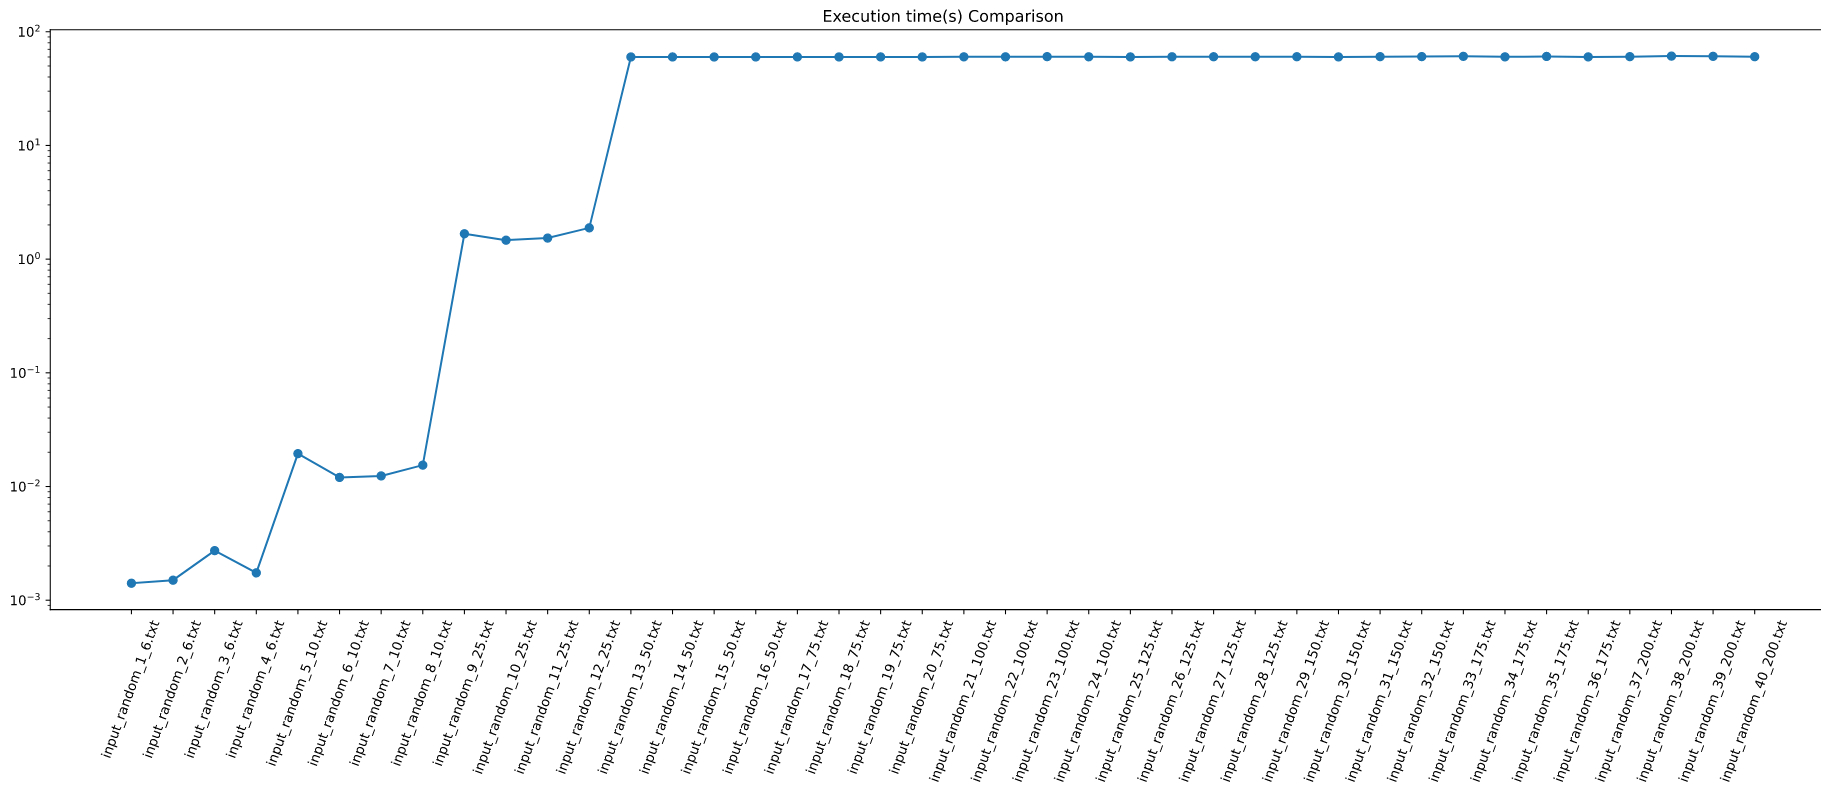
\includegraphics[width=\linewidth]{Img/exec_time_graph.jpg}
		\caption{Confronto dei tempi di esecuzione}
	\end{figure}
\end{center}

\subsection{Grafico di confronto dei tempi di Full Contraption}
\begin{center}
	\begin{figure}[H]
		\centering
		\hspace{-1cm}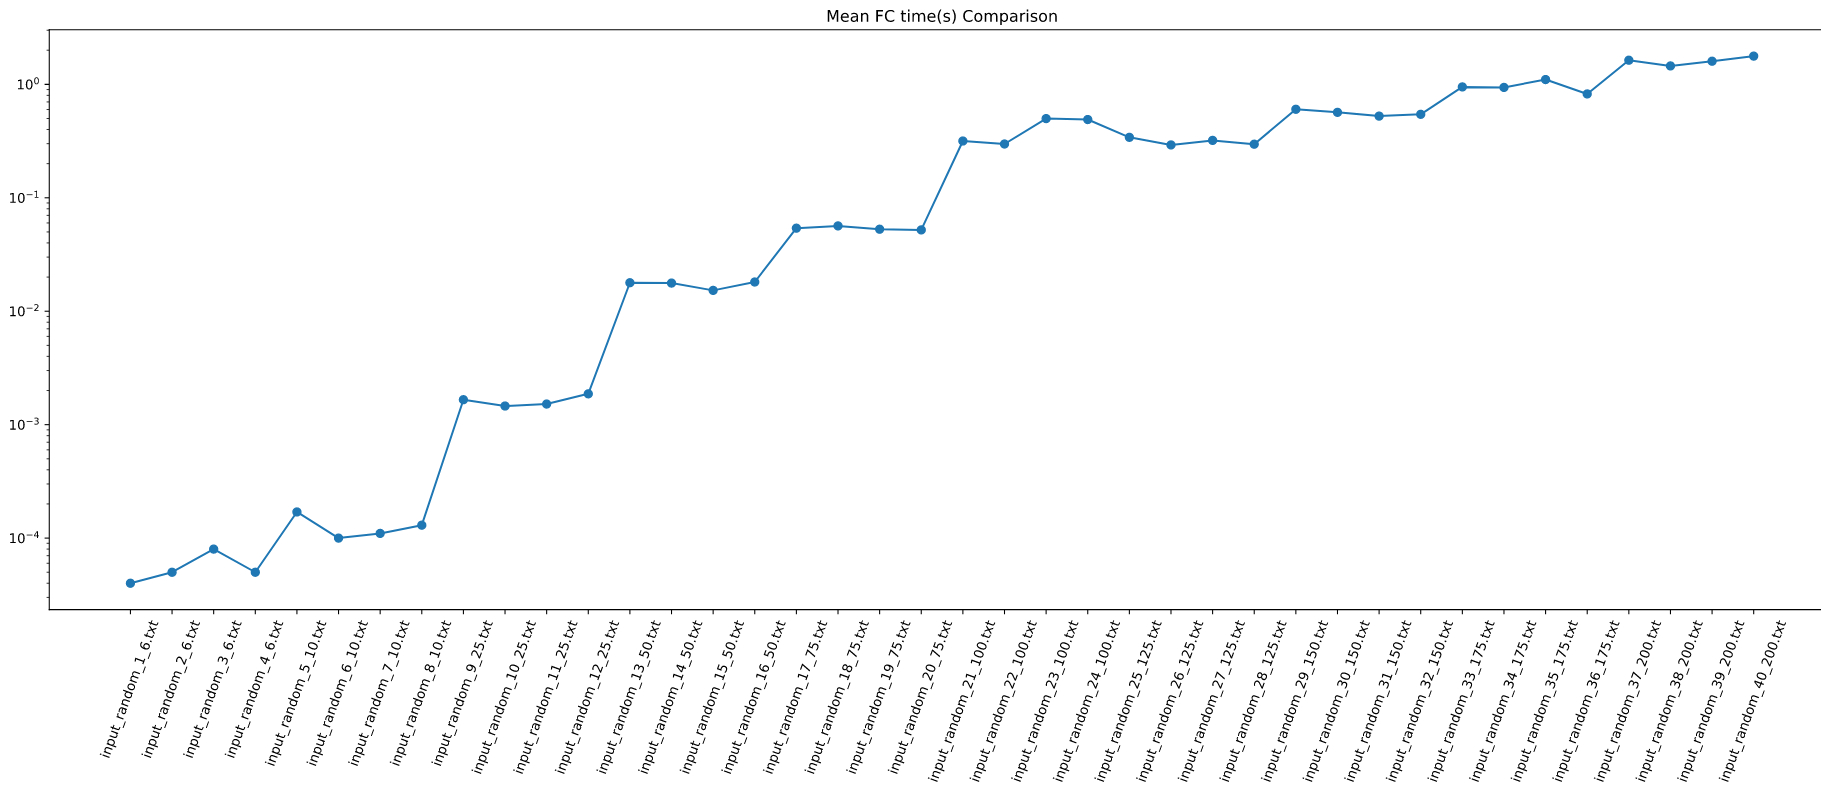
\includegraphics[width=\linewidth]{Img/fc_time_graph.jpg}
		\caption{Confronto dei tempi di Full Contraption}
	\end{figure}
\end{center}

\subsection{Grafico di confronto dei Discovery Time}
\begin{center}
	\begin{figure}[H]
		\centering
		\hspace{-1cm}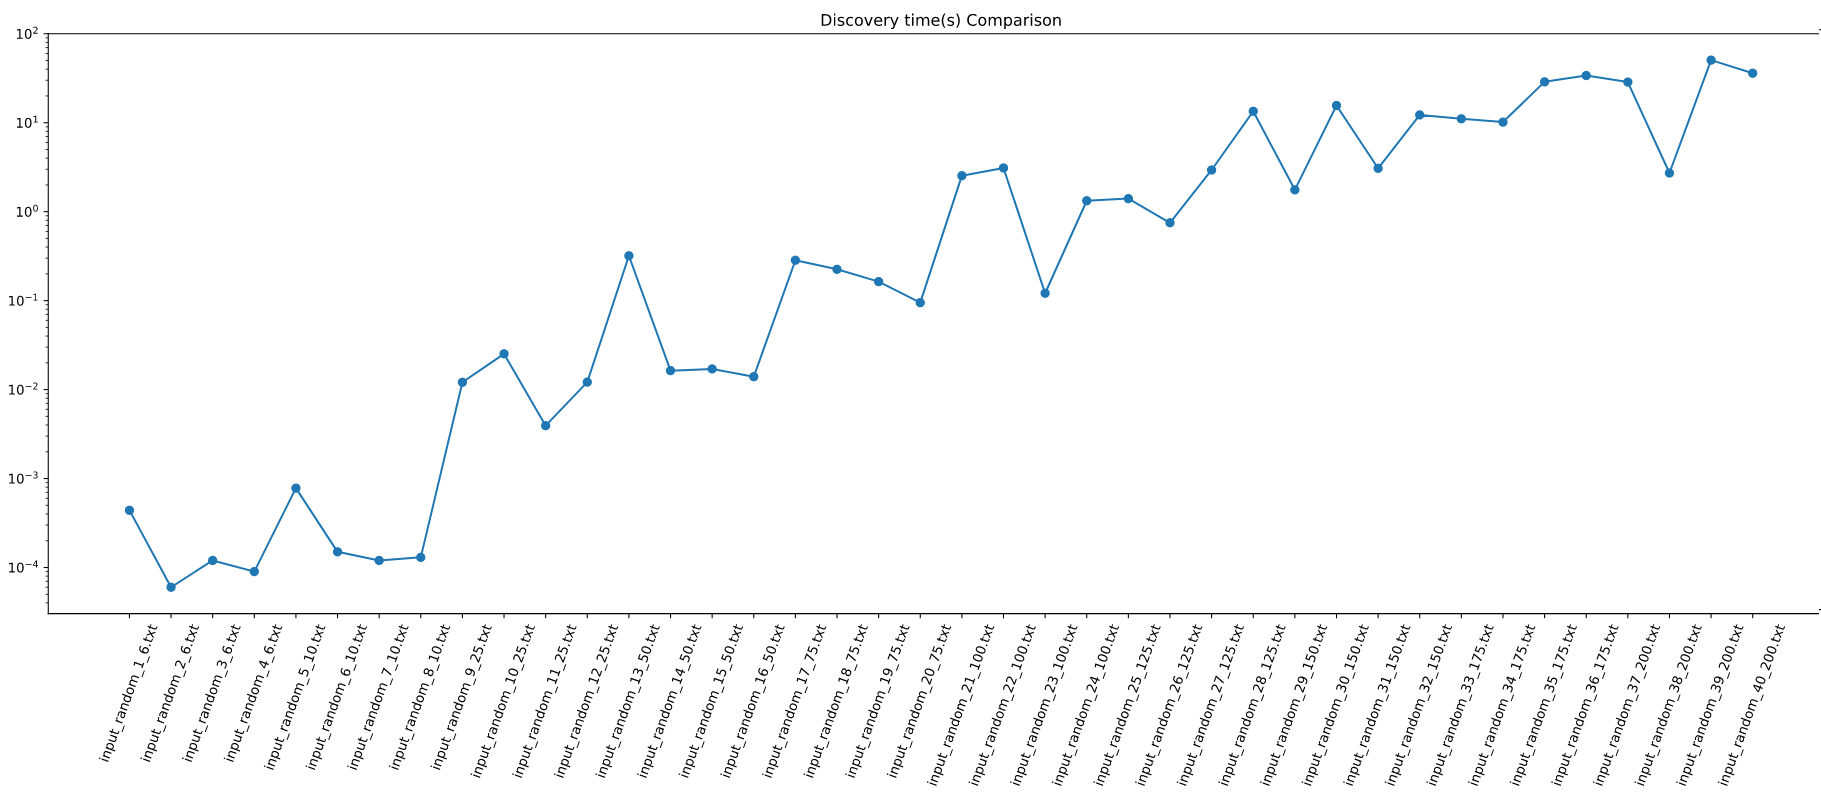
\includegraphics[width=\linewidth]{Img/disc_time_graph.jpg}
		\caption{Confronto dei Discovery Time}
	\end{figure}
\end{center}

\subsection{Grafico di confronto delle percentuali di errore}
\begin{center}
	\begin{figure}[H]
		\centering
		\hspace{-1cm}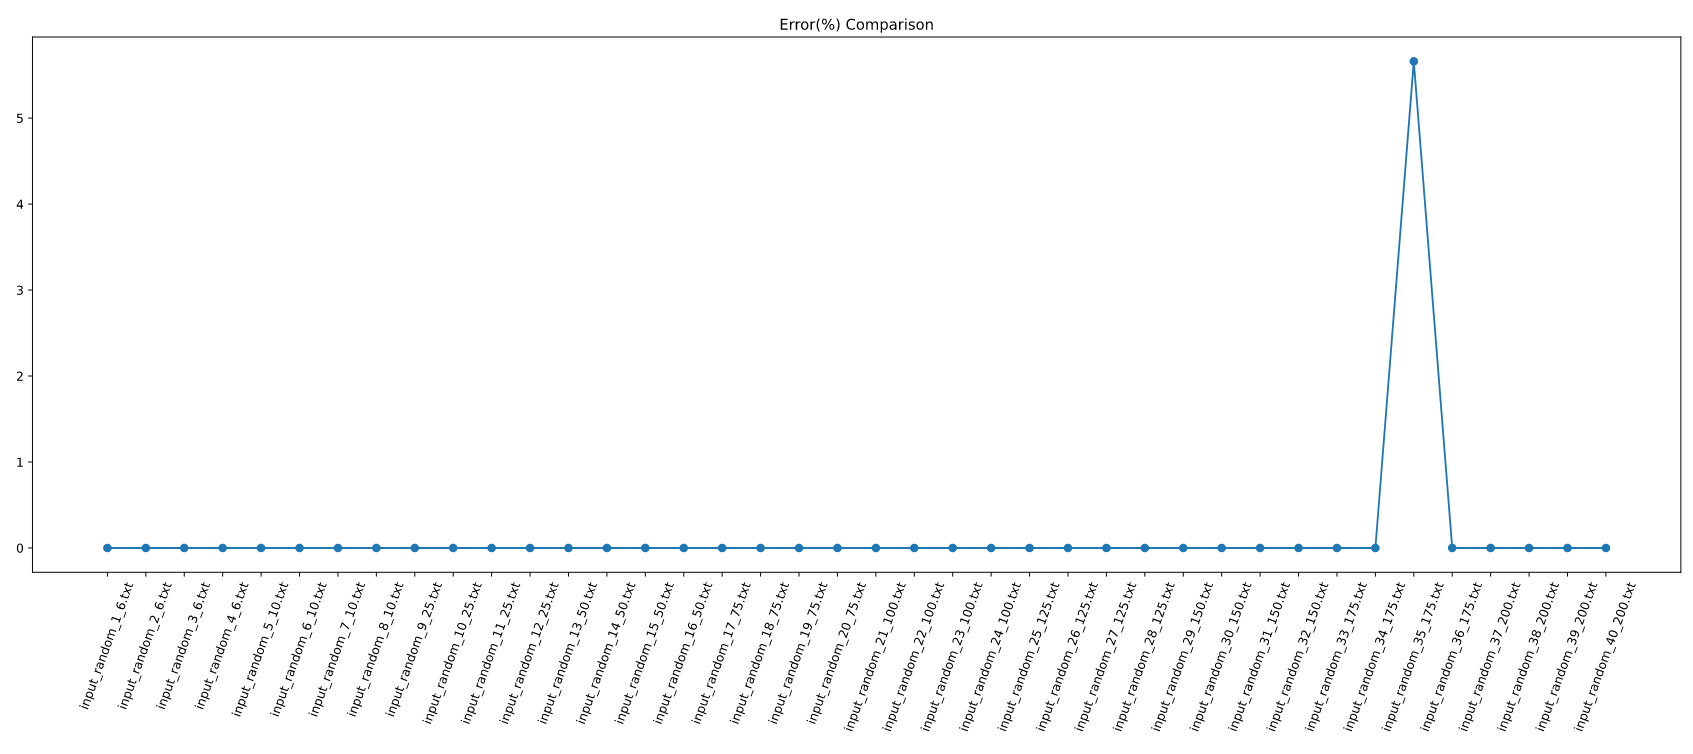
\includegraphics[width=\linewidth]{Img/err_perc_graph.jpg}
		\caption{Confronto delle percentuali di errore}
	\end{figure}
\end{center}

\pagebreak